\documentclass[aspectratio=169, 10pt]{beamer}
% =============================================================
% preamble.tex – G25 Metric Learning for Face Recognition
% Deep Learning: Advanced Models and Methods (DL26)
% =============================================================

% ---- Encoding & Language ----
\usepackage[T1]{fontenc}
\usepackage[utf8]{inputenc}
\usepackage[italian]{babel}

% ---- Font ----
\usepackage{lmodern}
\renewcommand{\familydefault}{\sfdefault}

% ---- Mathematics ----
\usepackage{amsmath}
\usepackage{amssymb}

% ---- Graphics ----
\usepackage{graphicx}
\graphicspath{{../../figures/}}

% ---- Color ----
\usepackage{xcolor}

\definecolor{colPrimary}{HTML}{1B3A5C}      % Deep Navy
\definecolor{colAccent}{HTML}{2E86AB}       % Steel Teal
\definecolor{colHighlight}{HTML}{E8832A}    % Warm Orange
\definecolor{colBg}{HTML}{F4F7FA}           % Light Gray
\definecolor{colText}{HTML}{3A3A4A}         % Dark Slate
\definecolor{colGreen}{HTML}{27AE60}        % Success Green
\definecolor{colRed}{HTML}{C0392B}          % Alert Red

% ---- TikZ ----
\usepackage{tikz}
\usetikzlibrary{arrows.meta, positioning, shapes.geometric, calc, decorations.pathreplacing}

% ---- Tables ----
\usepackage{booktabs}
\usepackage{array}
\usepackage{colortbl}

% ---- Misc ----
\usepackage{microtype}

% ================================================================
% BEAMER THEME
% ================================================================

\usetheme{default}
\usecolortheme{default}
\setbeamertemplate{navigation symbols}{}

% -- Structure --
\setbeamercolor{structure}{fg=colPrimary}
\setbeamercolor{frametitle}{bg=colPrimary, fg=white}
\setbeamercolor{normal text}{fg=colText, bg=white}
\setbeamercolor{alerted text}{fg=colHighlight}
\setbeamercolor{example text}{fg=colGreen}

% -- Blocks --
\setbeamercolor{block title}{bg=colAccent, fg=white}
\setbeamercolor{block body}{bg=colAccent!11!white, fg=colText}
\setbeamercolor{block title alerted}{bg=colHighlight, fg=white}
\setbeamercolor{block body alerted}{bg=colHighlight!11!white, fg=colText}
\setbeamercolor{block title example}{bg=colGreen!80!black, fg=white}
\setbeamercolor{block body example}{bg=colGreen!10!white, fg=colText}

% -- Head/foot (used in footer) --
\setbeamercolor{author in head/foot}{bg=colPrimary!88!black, fg=white!78!colPrimary}
\setbeamercolor{date in head/foot}{bg=colPrimary!92!black, fg=white}

% -- Fonts --
\setbeamerfont{frametitle}{size=\large, series=\bfseries}
\setbeamerfont{block title}{size=\small, series=\bfseries}
\setbeamerfont{itemize/enumerate body}{size=\small}
\setbeamerfont{itemize/enumerate subbody}{size=\footnotesize}

% -- Bullets --
\setbeamertemplate{itemize item}{%
    \color{colAccent}\raisebox{0.05em}{$\blacktriangleright$}\hspace{0.1em}}
\setbeamertemplate{itemize subitem}{%
    \color{colAccent!70!colText}\textbullet\hspace{0.1em}}
\setbeamertemplate{enumerate item}{%
    \color{colAccent}\bfseries\insertenumlabel.\hspace{0.2em}}

% -- Frame title --
\setbeamertemplate{frametitle}{%
    \begin{beamercolorbox}[wd=\paperwidth, ht=0.62cm, dp=0.14cm, leftskip=0.45cm]{frametitle}%
        \usebeamerfont{frametitle}\strut\insertframetitle%
    \end{beamercolorbox}%
}

% -- Footer --
\setbeamertemplate{footline}{%
    \leavevmode%
    \hbox{%
        \begin{beamercolorbox}[wd=.72\paperwidth, ht=2.1ex, dp=0.9ex,
                               leftskip=0.5em]{author in head/foot}%
            \tiny G25\enspace$\cdot$\enspace
            Metric Learning for Face Recognition\enspace$\cdot$\enspace DL26
        \end{beamercolorbox}%
        \begin{beamercolorbox}[wd=.28\paperwidth, ht=2.1ex, dp=0.9ex,
                               rightskip=0.5em, right]{date in head/foot}%
            \tiny \insertframenumber\,/\,\inserttotalframenumber
        \end{beamercolorbox}%
    }%
    \vskip0pt%
}

% ================================================================
% CUSTOM COMMANDS
% ================================================================
\newcommand{\good}[1]{{\color{colGreen}\textbf{#1}}}
\newcommand{\bad}[1]{{\color{colRed}\textbf{#1}}}
\newcommand{\warn}[1]{{\color{colHighlight}\textbf{#1}}}
\newcommand{\emphc}[1]{{\color{colPrimary}\textbf{#1}}}
\newcommand{\repo}{\texttt{github.com/MattiaCampanella/ml-face-recognition}}

% ================================================================
% TIKZ STYLES
% ================================================================
\tikzset{
    mybox/.style={
        draw=#1, fill=#1!13!white,
        rounded corners=3pt,
        minimum height=0.68cm,
        align=center,
        font=\scriptsize
    },
    mybox/.default=colAccent,
    myarrow/.style={-Stealth, thick, color=colText!55!white},
}


% ================================================================
% METADATA
% ================================================================
\title{Metric Learning per il Riconoscimento Facciale}
\subtitle{Track 1 – Deep Learning: Advanced Models and Methods (DL26)}
\author{Mattia Campanella \\ {\small Gruppo G25}}
\institute{}
\date{\texttt{github.com/MattiaCampanella/ml-face-recognition}}

\begin{document}

% ================================================================
% SLIDE 1 — COVER (obbligatoria, non conteggiata)
% ================================================================
\begin{frame}[plain, noframenumbering]
    \begin{tikzpicture}[remember picture, overlay]
        % Sfondo navy
        \fill[colPrimary]
            (current page.north west) rectangle (current page.south east);
        % Barra accent in basso
        \fill[colAccent]
            (current page.south west) rectangle ++(\paperwidth, 0.75cm);
        % Cerchi decorativi
        \fill[colAccent!35!colPrimary, opacity=0.22]
            ([xshift=2.2cm, yshift=-2.2cm]current page.north east) circle (5.8cm);
        \fill[white, opacity=0.04]
            ([xshift=-1.5cm, yshift=1.5cm]current page.south west) circle (4.5cm);
    \end{tikzpicture}
    %
    \vspace{0.9cm}
    \begin{center}
        {\color{white!52!colPrimary}\scriptsize\textsc{%
            Deep Learning: Advanced Models and Methods — DL26}}\\[0.55em]
        {\color{colAccent!80!white}\footnotesize
            Track 1 – Metric Learning for Face Recognition}\\[1.5em]
        {\color{white}\Large\bfseries
            Metric Learning per il Riconoscimento Facciale}\\[1.3em]
        \begin{tikzpicture}
            \draw[colAccent, line width=1.3pt] (0,0) -- (7cm,0);
        \end{tikzpicture}\\[1.0em]
        {\color{white!82!colPrimary}\normalsize
            Mattia Campanella\quad$\cdot$\quad Gruppo G25}\\[0.5em]
        {\color{colAccent!62!white}\small\repo}
    \end{center}
\end{frame}

% ================================================================
% SLIDE 2 — HOOK: Il problema
% ================================================================
\begin{frame}{Come riconosci un volto che non hai mai visto?}
\begin{columns}[T, onlytextwidth]

%% ---------- colonna sinistra ----------
\begin{column}{0.56\textwidth}
    \textbf{Il limite dei classificatori tradizionali}\\[0.35em]
    {\small Un modello addestrato su $N$ identità non può generalizzare
    su identità \warn{mai viste}: le feature sono ancorate alle classi
    di training, non alla geometria del volto.}

    \medskip
    \textbf{La soluzione: Metric Learning}\\[0.25em]
    {\small Impariamo $f:\mathcal{I}\to\mathbb{R}^{512}$ tale che:
    \[
      d\!\left(f(x_i),f(x_j)\right)\;\ll\; d\!\left(f(x_i),f(x_k)\right)
    \]
    quando $x_i,x_j$ sono la \good{stessa persona}
    e $x_k$ è una \bad{persona diversa}.}

    \medskip
    \begin{itemize}
        \item Variazioni di posa, illuminazione, espressione
        \item Generalizzazione \emphc{zero-shot} su nuove identità
        \item Valutazione: \emphc{mAP@1 / @5 / @10} su identità unseen
    \end{itemize}
\end{column}

%% ---------- colonna destra ----------
\begin{column}{0.40\textwidth}
    \centering
    \begin{tikzpicture}[scale=0.88]
        % Sfondo
        \fill[colBg] (-0.3,-0.3) rectangle (3.3,3.3);
        \draw[colText!14!white, very thin, step=0.5] (-0.3,-0.3) grid (3.3,3.3);
        % Persona A (teal)
        \foreach \px/\py in {0.38/0.48, 0.68/0.72, 0.50/0.92}{
            \fill[colAccent] (\px,\py) circle (4.5pt);}
        \draw[colAccent, dashed, opacity=0.55] (0.52,0.70) circle (0.50cm);
        \node[colAccent, font=\tiny\bfseries, below] at (0.52,0.12) {Persona A};
        % Persona B (green)
        \foreach \px/\py in {2.40/0.58, 2.68/0.38, 2.52/0.88}{
            \fill[colGreen] (\px,\py) circle (4.5pt);}
        \draw[colGreen, dashed, opacity=0.55] (2.53,0.62) circle (0.48cm);
        \node[colGreen, font=\tiny\bfseries, below] at (2.53,0.08) {Persona B};
        % Persona C (orange)
        \foreach \px/\py in {1.18/2.28, 1.48/2.08, 1.30/2.58}{
            \fill[colHighlight] (\px,\py) circle (4.5pt);}
        \draw[colHighlight, dashed, opacity=0.55] (1.32,2.32) circle (0.48cm);
        \node[colHighlight, font=\tiny\bfseries, above] at (1.32,2.88) {Persona C};
        % Assi
        \draw[-Stealth, colText!35!white, thin] (-0.3,-0.3) -- (3.45,-0.3);
        \draw[-Stealth, colText!35!white, thin] (-0.3,-0.3) -- (-0.3,3.45);
        \node[colText!45!white, font=\tiny, above] at (-0.3,3.45) {$\mathbb{R}^{512}$};
    \end{tikzpicture}

    \vspace{0.25cm}
    \begin{alertblock}{\small Obiettivo di valutazione}
        \small\textbf{mAP@1, @5, @10} su identità \textbf{unseen}\\
        (retrieval: trova il volto più simile)
    \end{alertblock}
\end{column}

\end{columns}
\end{frame}

% ================================================================
% SLIDE 3 — DATASET: CASIA-WebFace
% ================================================================
\begin{frame}{CASIA-WebFace: grande, ricco, e con un'insidia nascosta}
\begin{columns}[T, onlytextwidth]

%% ---------- colonna sinistra ----------
\begin{column}{0.50\textwidth}
    \begin{block}{Il Dataset}
        \small\renewcommand{\arraystretch}{1.25}
        \begin{tabular}{@{}ll@{}}
            \toprule
            \textbf{Caratteristica} & \textbf{Valore} \\
            \midrule
            Immagini totali  & $\approx$490.000 \\
            Identità uniche  & $\approx$10.000  \\
            Formato originale & MXNet RecordIO  \\
            \bottomrule
        \end{tabular}
    \end{block}

    \medskip
    \textbf{Split per identità disgiunte} (zero leakage):\\[0.4em]
    \begin{tikzpicture}[font=\scriptsize, node distance=0.5cm and 0.25cm]
        \node[mybox=colPrimary, minimum width=3.8cm] (ds)
              {CASIA-WebFace};
        \node[mybox=colAccent, minimum width=1.65cm,
              below left=0.60cm and -0.15cm of ds] (tr)
              {\shortstack{Train\\(seen IDs)}};
        \node[mybox=colHighlight, minimum width=1.65cm,
              below right=0.60cm and -0.15cm of ds] (te)
              {\shortstack{Val / Test\\(unseen IDs)}};
        \draw[myarrow] (ds.south west) -- (tr.north);
        \draw[-Stealth, thick, color=colHighlight!65!colText] (ds.south east) -- (te.north);
        \node[color=colRed, font=\tiny, below=0.06cm of te] {zero identity overlap};
    \end{tikzpicture}
\end{column}

%% ---------- colonna destra ----------
\begin{column}{0.46\textwidth}
    \begin{alertblock}{\warn{[!]} Label Noise — problema critico}
        \small
        Studi scientifici (\emph{Anti-noise}, CVPR) stimano in CASIA:
        \begin{itemize}
            \item \bad{9.3\%–13\%} di sample rumorosi o errati
            \item \bad{7.7\%} di \textbf{mislabeling} effettivo
        \end{itemize}
        \medskip
        \emphc{Impatto diretto} sul training con hard mining:\\
        i falsi negativi avvelenano il gradiente.
    \end{alertblock}

    \medskip
    {\small\textbf{Perché è critico?}\\[0.2em]
    Con hard mining il modello cerca attivamente i casi più
    difficili. Se sono rumorosi, distruggono il segnale
    di apprendimento — lo vedremo nella slide successiva.}
\end{column}

\end{columns}
\end{frame}

% ================================================================
% SLIDE 4 — BASELINE
% ================================================================
\begin{frame}{Baseline: classificazione supervisionata come punto di partenza}
\begin{columns}[T, onlytextwidth]

%% ---------- colonna sinistra ----------
\begin{column}{0.54\textwidth}
    \textbf{Architettura}\\[0.45em]
    \begin{tikzpicture}[font=\scriptsize, node distance=0.2cm and 0.22cm]
        \node[mybox=colPrimary, minimum width=1.55cm] (img)
              {\shortstack{Input\\224$\times$224}};
        \node[mybox=colAccent, minimum width=1.55cm, right=0.32cm of img] (bb)
              {\shortstack{ResNet-18\\backbone}};
        \node[mybox=colAccent, minimum width=1.55cm, right=0.32cm of bb] (proj)
              {\shortstack{Linear\\512-d}};
        \node[mybox=colHighlight, minimum width=1.55cm, right=0.32cm of proj] (l2)
              {\shortstack{L2-norm\\embedding}};

        \draw[myarrow] (img) -- (bb);
        \draw[myarrow] (bb) -- (proj);
        \draw[myarrow] (proj) -- (l2);

        \node[color=colAccent!70!colText, font=\tiny, below=0.05cm of bb]
              {\shortstack{pretrained\\ImageNet}};
        \node[color=colHighlight!75!colText, font=\tiny, below=0.05cm of l2]
              {cosine sim.};

        % Training path (dashed)
        \node[mybox=colPrimary!55!white, minimum width=1.35cm,
              below=0.70cm of proj] (ce) {\shortstack{Cross-Entropy\\Loss}};
        \draw[-Stealth, dashed, color=colText!45!white] (proj.south) -- (ce.north)
              node[midway, right, font=\tiny] {train};

        % Inference path (dashed)
        \node[mybox=colGreen, minimum width=1.35cm,
              below=0.70cm of l2] (ret) {\shortstack{KNN\\Retrieval}};
        \draw[-Stealth, dashed, color=colGreen!65!colText] (l2.south) -- (ret.north)
              node[midway, right, font=\tiny] {inference};
    \end{tikzpicture}

    \medskip
    \begin{block}{\small Il limite concettuale}
        \small La Cross-Entropy ottimizza la separazione tra
        \emph{classi note}. L'embedding risultante \textbf{non è
        ottimizzato} per il retrieval su identità unseen.
    \end{block}
\end{column}

%% ---------- colonna destra ----------
\begin{column}{0.42\textwidth}
    \textbf{Risultati Baseline}\\[0.5em]
    \small\renewcommand{\arraystretch}{1.30}
    \begin{center}
    \begin{tabular}{lc}
        \toprule
        \textbf{Metrica} & \textbf{Score} \\
        \midrule
        mAP@1  & $\approx$63.0\% \\
        mAP@5  & $\approx$50.7\% \\
        mAP@10 & $\approx$44.1\% \\
        \bottomrule
    \end{tabular}
    \end{center}

    \medskip
    % Bar chart baseline
    \begin{tikzpicture}
        % Scale: 1% -> 0.027cm
        \fill[colAccent!48!white] (0.10,0) rectangle (0.52,1.701); % 63%
        \fill[colAccent!33!white] (0.70,0) rectangle (1.12,1.369); % 50.7%
        \fill[colAccent!18!white] (1.30,0) rectangle (1.72,1.191); % 44.1%
        % Value labels
        \node[font=\tiny, above] at (0.31,1.701) {63\%};
        \node[font=\tiny, above] at (0.91,1.369) {51\%};
        \node[font=\tiny, above] at (1.51,1.191) {44\%};
        % Axis labels
        \node[font=\tiny, below] at (0.31,-0.05) {mAP@1};
        \node[font=\tiny, below] at (0.91,-0.05) {mAP@5};
        \node[font=\tiny, below] at (1.51,-0.05) {mAP@10};
        % Y axis
        \draw[-Stealth, colText!25!white, thin] (0.0,0) -- (0.0,2.85);
        % Grid
        \draw[colText!12!white, thin] (0.0,0.675) -- (2.0,0.675);
        \node[font=\tiny, left, color=colText!45!white] at (0.0,0.675) {25\%};
        \draw[colText!12!white, thin] (0.0,1.350) -- (2.0,1.350);
        \node[font=\tiny, left, color=colText!45!white] at (0.0,1.350) {50\%};
        \draw[colText!12!white, thin] (0.0,2.025) -- (2.0,2.025);
        \node[font=\tiny, left, color=colText!45!white] at (0.0,2.025) {75\%};
        \draw[colText!12!white, thin] (0.0,2.700) -- (2.0,2.700);
        \node[font=\tiny, left, color=colText!45!white] at (0.0,2.700) {100\%};
    \end{tikzpicture}

    \smallskip
    {\small\warn{Ampio margine di miglioramento} $\to$ metric learning}
\end{column}

\end{columns}
\end{frame}

% ================================================================
% SLIDE 5 — METODO: Triplet Loss + PK Sampling
% ================================================================
\begin{frame}{Il metodo: Triplet Loss con PK Sampling e Online Hard Mining}
\begin{columns}[T, onlytextwidth]

%% ---------- colonna sinistra ----------
\begin{column}{0.46\textwidth}
    \textbf{La Tripletta}\\[0.45em]
    \begin{tikzpicture}[font=\scriptsize, node distance=0.25cm]
        % Anchor
        \node[circle, draw=colPrimary, fill=colPrimary, text=white,
              minimum size=0.92cm, font=\small\bfseries] (A) {A};
        \node[below=0.05cm of A, colPrimary, font=\tiny] {Anchor};
        % Positive
        \node[circle, draw=colGreen, fill=colGreen, text=white,
              minimum size=0.92cm, font=\small\bfseries,
              above right=1.05cm and 2.20cm of A] (P) {P\!+};
        \node[above=0.05cm of P, colGreen, font=\tiny] {Positive (stessa ID)};
        % Negative
        \node[circle, draw=colRed, fill=colRed, text=white,
              minimum size=0.92cm, font=\small\bfseries,
              below right=1.05cm and 2.20cm of A] (N) {N\!-};
        \node[below=0.05cm of N, colRed, font=\tiny] {Negative (altra ID)};
        % Frecce
        \draw[-Stealth, colGreen, thick] (A.north east) -- (P.west)
              node[midway, above, sloped, font=\tiny] {\good{vicini}};
        \draw[-Stealth, colRed, thick] (A.south east) -- (N.west)
              node[midway, below, sloped, font=\tiny] {\bad{lontani}};
    \end{tikzpicture}

    \medskip
    \textbf{PK Sampling — batch efficaci:}
    \begin{itemize}
        \item $P = 32$ identità $\times$ $K = 4$ immagini/ID
        \item Batch effettivo: $128$ immagini bilanciate
        \item Garantisce mining \emphc{ricco e stabile}
    \end{itemize}
\end{column}

%% ---------- colonna destra ----------
\begin{column}{0.50\textwidth}
    \textbf{Online Mining batch-wise}\\[0.35em]
    \small
    \begin{enumerate}
        \item Estrai embedding per il batch (128 immagini)
        \item Calcola matrice distanze $D\in\mathbb{R}^{128\times128}$ (cosine)
        \item Per ogni anchor seleziona:
        \begin{itemize}
            \item \warn{Hard positive}: positivo \emph{più lontano}
            \item \warn{Hard negative}: negativo \emph{più vicino}
        \end{itemize}
        \item Calcola la loss solo sui triplet difficili
    \end{enumerate}

    \medskip
    \begin{block}{\small Perché hard mining?}
        \small I triplet \emph{easy} producono gradiente $\approx 0$:\\
        il modello non impara nulla da essi.\\
        Hard mining seleziona i casi più \emphc{informativi}.
    \end{block}

    \medskip
    {\small Distanza usata:
    $d(u,v) = 1 - \langle u,v\rangle$
    su embedding L2-normalizzati.}
\end{column}

\end{columns}
\end{frame}

% ================================================================
% SLIDE 6 — SOFT vs HINGE
% ================================================================
\begin{frame}{La formulazione della loss conta più del margine: soft batte hinge}
\begin{columns}[T, onlytextwidth]

%% ---------- colonna sinistra ----------
\begin{column}{0.47\textwidth}
    \begin{alertblock}{\bad{[X]} Hinge — instabile con label noise}
        \[
          \mathcal{L}_{\mathrm{hinge}} =
          \max\!\bigl(0,\; d^{+} - d^{-} + m\bigr)
        \]
        {\small Margine esplicito $m$: i mislabeled CASIA diventano
        falsi hard negative e \textbf{avvelenano il gradiente} $\to$
        collasso del modello.}
    \end{alertblock}

    \medskip
    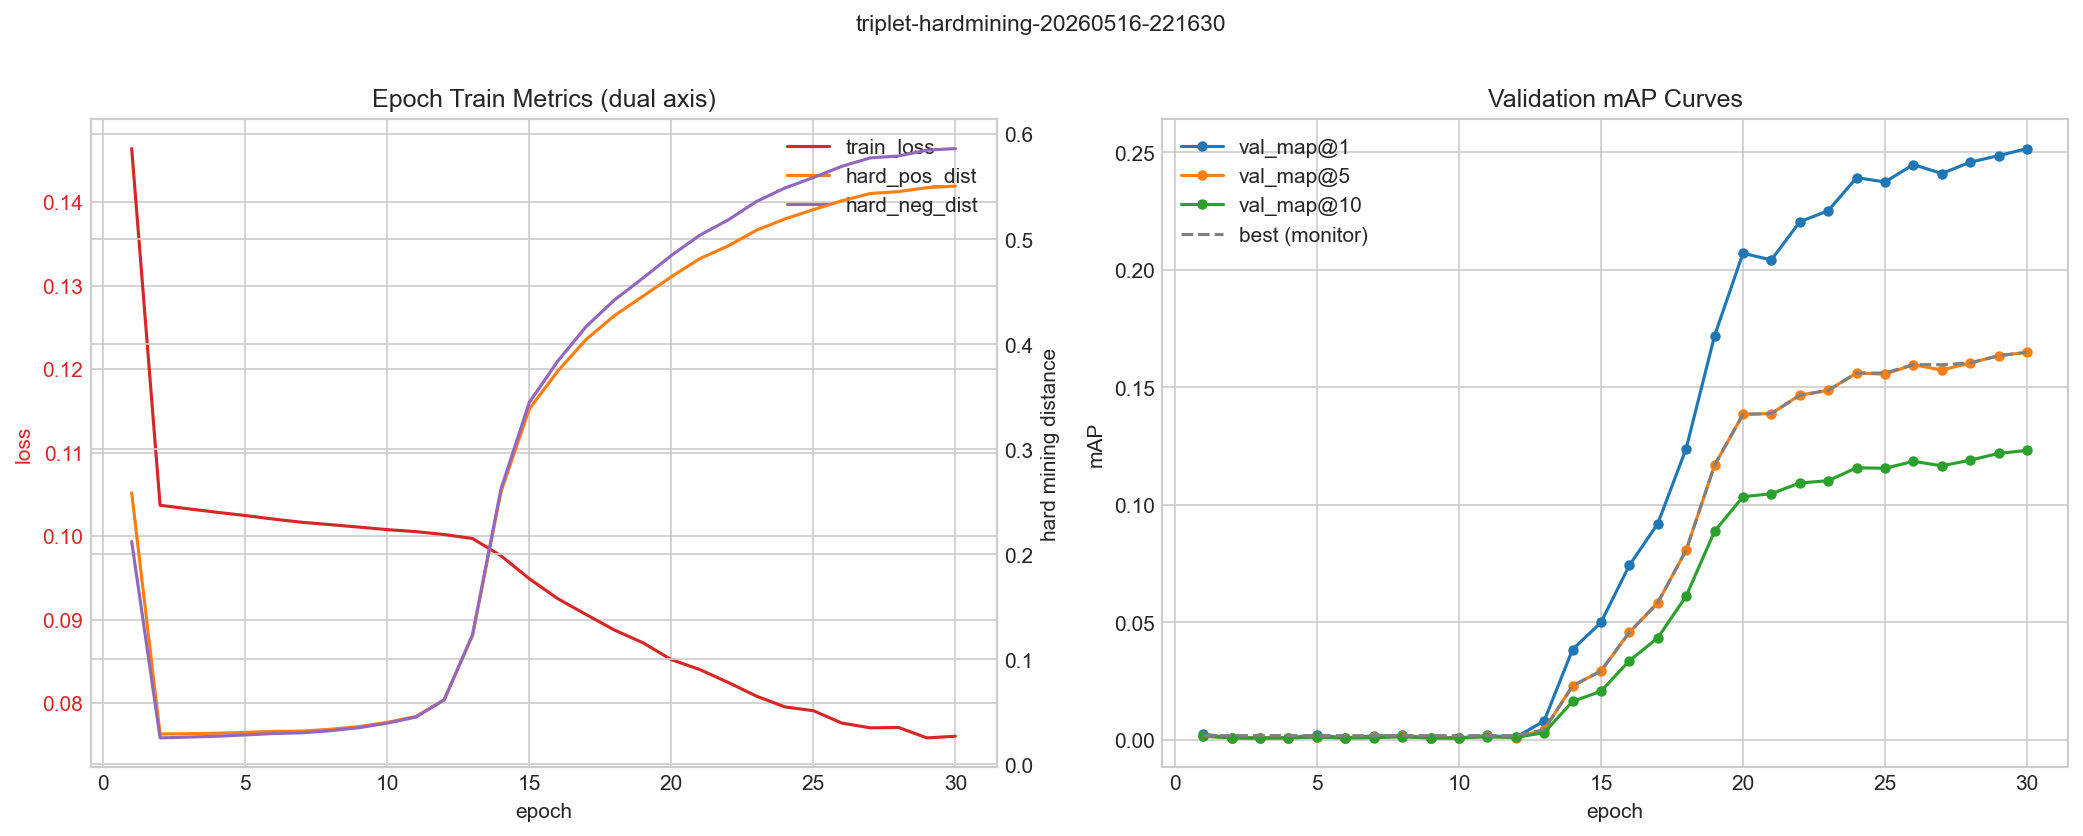
\includegraphics[width=\linewidth, height=3.5cm,
                     keepaspectratio]{hinge.png}\\
    {\tiny\centering\color{colText!55!white}
        Curve hinge + hard mining: collasso visibile\par}
\end{column}

%% ---------- colonna destra ----------
\begin{column}{0.47\textwidth}
    \begin{exampleblock}{\good{[OK]} Softplus — robusta al rumore}
        \[
          \mathcal{L}_{\mathrm{soft}} =
          \log\!\Bigl(1 + e^{\,d^{+} - d^{-}}\Bigr)
        \]
        {\small Nessun margine fisso: penalizzazione continua e
        proporzionale. Tollerante al noise $\to$ convergenza
        stabile.}
    \end{exampleblock}

    \medskip
    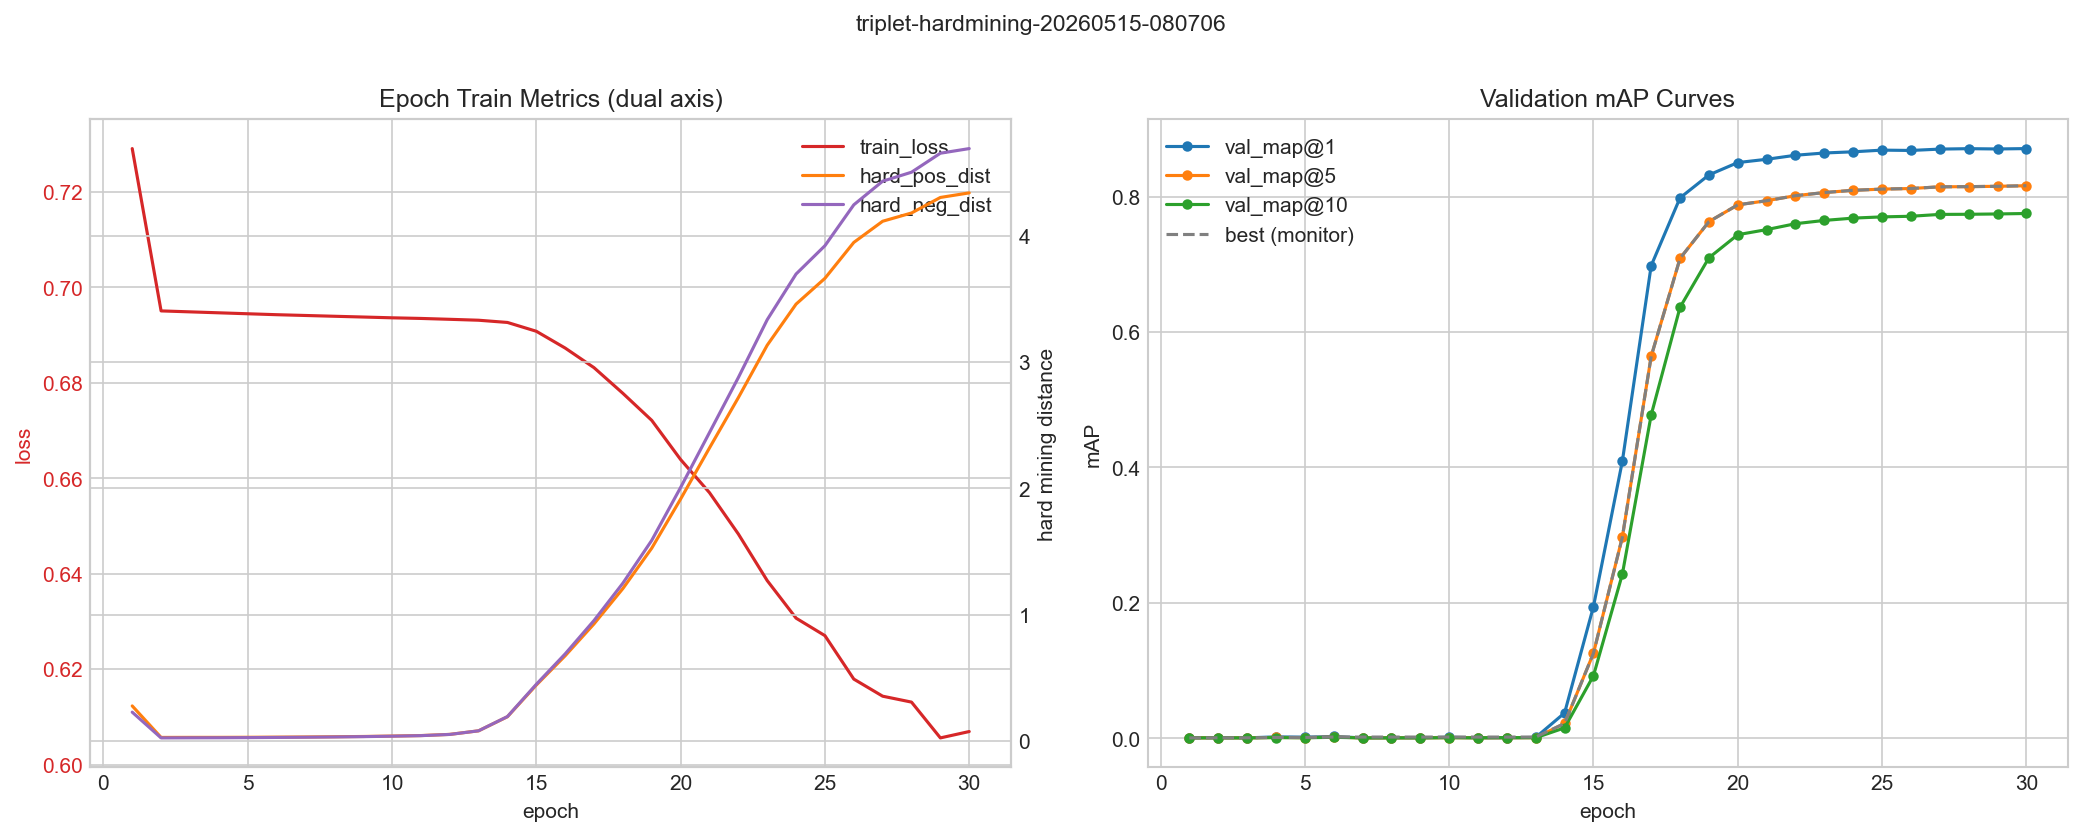
\includegraphics[width=\linewidth, height=3.5cm,
                     keepaspectratio]{soft.png}\\
    {\tiny\centering\color{colText!55!white}
        Curve softmargin + hard mining: convergenza pulita\par}
\end{column}

\end{columns}

\vspace{0.30cm}
\centering
{\small\color{colPrimary}
Con il \emphc{13\% di label noise} di CASIA, la formulazione
\emph{soft} non è solo migliore:
è \textbf{necessaria} per la stabilità del training.}
\end{frame}

% ================================================================
% SLIDE 7 — RISULTATI
% ================================================================
\begin{frame}{+24 p.p. di mAP@1: il metric learning supera nettamente il baseline}
\begin{columns}[T, onlytextwidth]

%% ---------- colonna sinistra ----------
\begin{column}{0.52\textwidth}
    \small\renewcommand{\arraystretch}{1.40}
    \begin{center}
    \begin{tabular}{lccc}
        \toprule
        \textbf{Modello} & \textbf{@1} & \textbf{@5} & \textbf{@10} \\
        \midrule
        Baseline (CE)         & 63.0\% & 50.7\% & 44.1\% \\
        \rowcolor{colGreen!18!white}
        \textbf{Triplet Soft} & \textbf{87.0\%} & \textbf{81.0\%} & \textbf{77.0\%} \\
        ArcFace               & 82.1\% & 74.6\% & 69.0\% \\
        \bottomrule
    \end{tabular}
    \end{center}

    \medskip
    \textbf{Cosa emerge:}
    \begin{enumerate}
        \item \good{+24 p.p.} di mAP@1 rispetto al baseline
        \item Triplet Soft \good{supera ArcFace} di +4.9 p.p. @1
        \item ArcFace comunque \good{+19 p.p.} vs baseline
    \end{enumerate}

    \medskip
    {\small\color{colText!65!white}
    Il vantaggio è frutto dell'interazione tra
    \emphc{soft loss} + \emphc{hard mining} + \emphc{PK(32,4)},
    non di un singolo iperparametro.}
\end{column}

%% ---------- colonna destra ----------
\begin{column}{0.44\textwidth}
    \centering
    % Grouped bar chart — hardcoded per evitare ambiguità TikZ
    % Scale: 1% -> 0.028cm  |  bar width: 0.26cm  |  gap: 0.05cm
    \begin{tikzpicture}
        % === Group @1 (starts x=0.10) ===
        \fill[colAccent!45!white]    (0.10,0) rectangle (0.36,1.764); % 63%
        \fill[colGreen!80!white]     (0.41,0) rectangle (0.67,2.436); % 87%
        \fill[colHighlight!65!white] (0.72,0) rectangle (0.98,2.299); % 82.1%
        % === Group @5 (starts x=1.32) ===
        \fill[colAccent!45!white]    (1.32,0) rectangle (1.58,1.420); % 50.7%
        \fill[colGreen!80!white]     (1.63,0) rectangle (1.89,2.268); % 81%
        \fill[colHighlight!65!white] (1.94,0) rectangle (2.20,2.089); % 74.6%
        % === Group @10 (starts x=2.54) ===
        \fill[colAccent!45!white]    (2.54,0) rectangle (2.80,1.235); % 44.1%
        \fill[colGreen!80!white]     (2.85,0) rectangle (3.11,2.156); % 77%
        \fill[colHighlight!65!white] (3.16,0) rectangle (3.42,1.932); % 69%

        % Etichette gruppi
        \node[font=\tiny, below] at (0.54,-0.06) {mAP@1};
        \node[font=\tiny, below] at (1.76,-0.06) {mAP@5};
        \node[font=\tiny, below] at (2.98,-0.06) {mAP@10};

        % Asse Y
        \draw[-Stealth, colText!22!white, thin] (0.02,0) -- (0.02,2.95);
        % Griglia
        \draw[colText!10!white, thin] (0.05,0.700) -- (3.55,0.700);
        \node[font=\tiny, left, color=colText!45!white] at (0.02,0.700) {25\%};
        \draw[colText!10!white, thin] (0.05,1.400) -- (3.55,1.400);
        \node[font=\tiny, left, color=colText!45!white] at (0.02,1.400) {50\%};
        \draw[colText!10!white, thin] (0.05,2.100) -- (3.55,2.100);
        \node[font=\tiny, left, color=colText!45!white] at (0.02,2.100) {75\%};

        % Legenda
        \fill[colAccent!45!white]    (0.10,2.72) rectangle (0.32,2.84);
        \node[right, font=\tiny] at (0.34,2.78) {Baseline};
        \fill[colGreen!80!white]     (1.10,2.72) rectangle (1.32,2.84);
        \node[right, font=\tiny] at (1.34,2.78) {Triplet};
        \fill[colHighlight!65!white] (2.10,2.72) rectangle (2.32,2.84);
        \node[right, font=\tiny] at (2.34,2.78) {ArcFace};

        % Annotazione +24pp
        \draw[colGreen, thin, -Stealth]
            (0.23,1.764) -- (0.23,2.436)
            node[midway, right, font=\tiny, color=colGreen] {+24pp};
        \draw[colGreen, thin, -Stealth]
            (0.23,2.436) -- (0.23,1.764);
    \end{tikzpicture}
\end{column}

\end{columns}
\end{frame}

% ================================================================
% SLIDE 8 — SPAZIO LATENTE
% ================================================================
\begin{frame}{Lo spazio latente si organizza: cluster compatti per identità}
\begin{columns}[T, onlytextwidth]

%% ---------- colonna sinistra ----------
\begin{column}{0.46\textwidth}
    \centering
    {\small\bfseries t-SNE degli embedding (Triplet Soft)}\\[0.25em]
    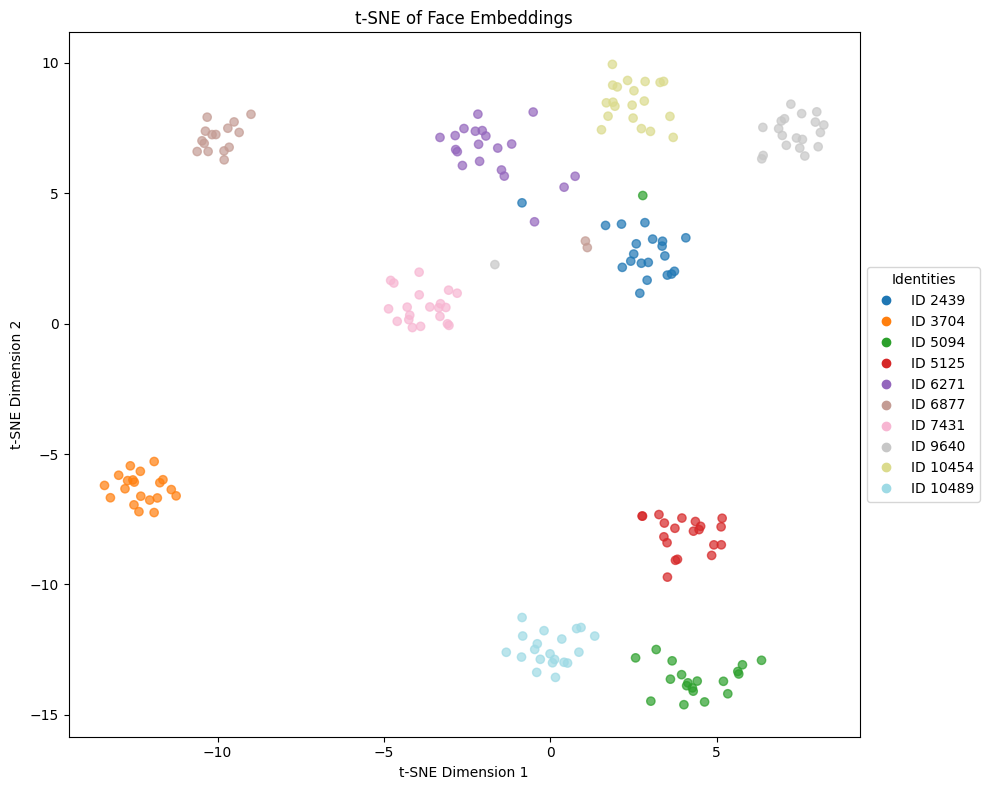
\includegraphics[width=0.96\linewidth, height=4.2cm,
                     keepaspectratio]{tsne_triplet.png}

    \smallskip
    {\small\bfseries PCA degli embedding (Triplet Soft)}\\[0.25em]
    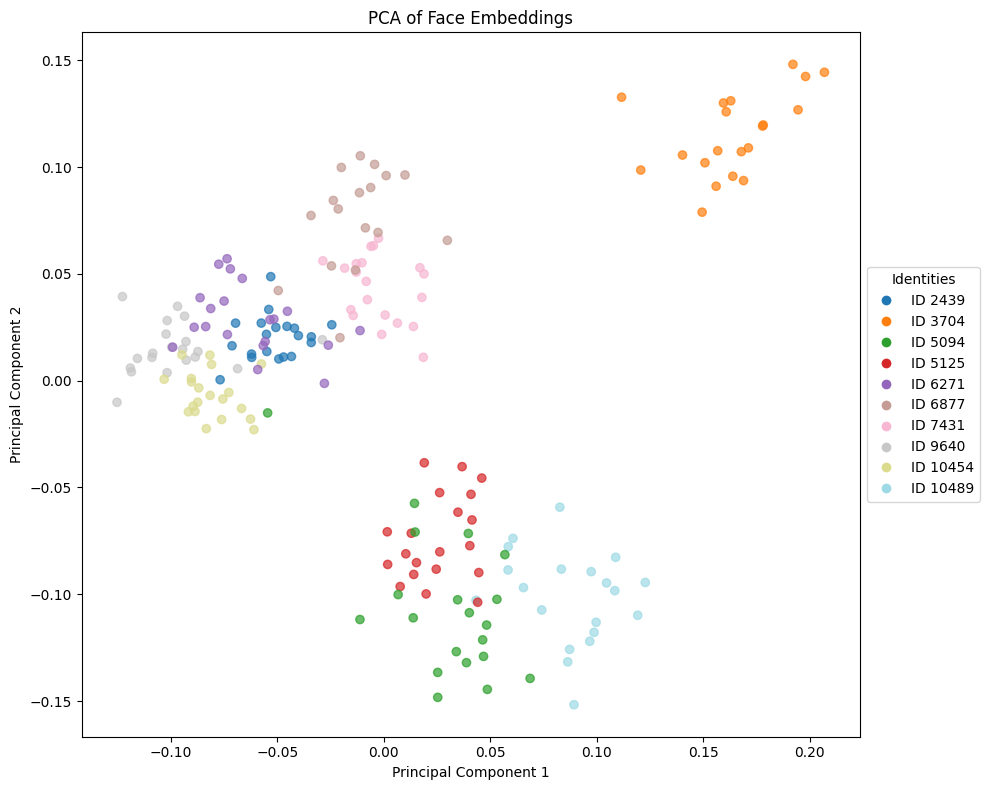
\includegraphics[width=0.96\linewidth, height=2.8cm,
                     keepaspectratio]{pca_triplet.png}
\end{column}

%% ---------- colonna destra ----------
\begin{column}{0.50\textwidth}
    \textbf{Cosa mostrano i plot}:\\[0.3em]
    \begin{itemize}
        \item Cluster \good{compatti e separati} per identità
        \item Spazio coseno \good{ben strutturato} $\to$ retrieval efficace
        \item Rispetto al baseline: embedding più \warn{dispersi e sovrapposti}
    \end{itemize}

    \medskip
    \textbf{Le training curve confermano}:\\[0.3em]
    \begin{itemize}
        \item \good{Softmargin}: $d^-$ cresce stabilmente,\\
              $d^+$ si riduce gradualmente
        \item \bad{Hingemargin}: $d^+$ diverge in corrispondenza\\
              dei sample rumorosi $\to$ collasso
    \end{itemize}

    \medskip
    \begin{block}{\small Validazione qualitativa}
        \small L'analisi visiva corrobora i numeri di mAP:\\
        le identità si separano nello spazio degli embedding
        L2-normalizzati a 512 dimensioni.
    \end{block}
\end{column}

\end{columns}
\end{frame}

% ================================================================
% SLIDE 9 — CONCLUSIONI
% ================================================================
\begin{frame}{Conclusioni: soft mining + PK batch = +24 p.p. zero-shot}
\begin{columns}[T, onlytextwidth]

%% ---------- colonna sinistra ----------
\begin{column}{0.54\textwidth}
    \begin{exampleblock}{\good{[OK]} Messaggio principale}
        \small
        Il Triplet con \emphc{soft loss} e \emphc{PK(32,4)} porta il mAP@1
        \textbf{dal 63\% all'87\%}, superando anche ArcFace
        (+4.9 p.p.)\\[0.3em]
        La chiave: la formulazione \emph{soft} è più importante
        del valore del margine, specialmente con dataset rumorosi.
    \end{exampleblock}

    \medskip
    \textbf{3 Takeaway concreti:}
    \begin{enumerate}
        \item \good{Soft $>$ Hinge} con label noise elevato:\\
              il margine esplicito è instabile con CASIA
        \item \good{PK(32,4) + hard mining} è il compromesso ottimale:\\
              batch più piccoli portano a overfitting
        \item \good{Hard mining è necessario}:\\
              mining easy/semi crea un gap di oltre 17 p.p.
    \end{enumerate}
\end{column}

%% ---------- colonna destra ----------
\begin{column}{0.42\textwidth}
    \begin{alertblock}{\warn{[!]} Limiti riconosciuti}
        \small
        \begin{itemize}
            \item \textbf{Mislabeling CASIA} (7.7\%–13\%):\\
                  avvelena il gradiente con hard mining
            \item \textbf{Assenza di Face Alignment}:\\
                  no MTCNN/landmark cropping\\
                  $\to$ variabilità non ridotta preventivamente
        \end{itemize}
    \end{alertblock}

    \medskip
    \textbf{Lavoro futuro:}
    \begin{itemize}
        \item Noise detection semi-supervisionata
        \item Sub-center ArcFace per cluster rumorosi
        \item Face alignment preprocessing (MTCNN)
    \end{itemize}
\end{column}

\end{columns}
\end{frame}

% ================================================================
% BACKUP SLIDE — Demo Website (non conteggiata nel timing)
% ================================================================
\appendix

\setbeamertemplate{footline}{%
    \leavevmode%
    \hbox{%
        \begin{beamercolorbox}[wd=.72\paperwidth, ht=2.1ex, dp=0.9ex,
                               leftskip=0.5em]{author in head/foot}%
            \tiny G25\enspace$\cdot$\enspace Backup — Demo Website
        \end{beamercolorbox}%
        \begin{beamercolorbox}[wd=.28\paperwidth, ht=2.1ex, dp=0.9ex,
                               rightskip=0.5em, right]{date in head/foot}%
            \tiny Backup
        \end{beamercolorbox}%
    }%
    \vskip0pt%
}

\begin{frame}{Demo Live: Riconoscimento in Azione}
\centering
\textbf{Demo live del modello disponibile online}\\[0.5em]
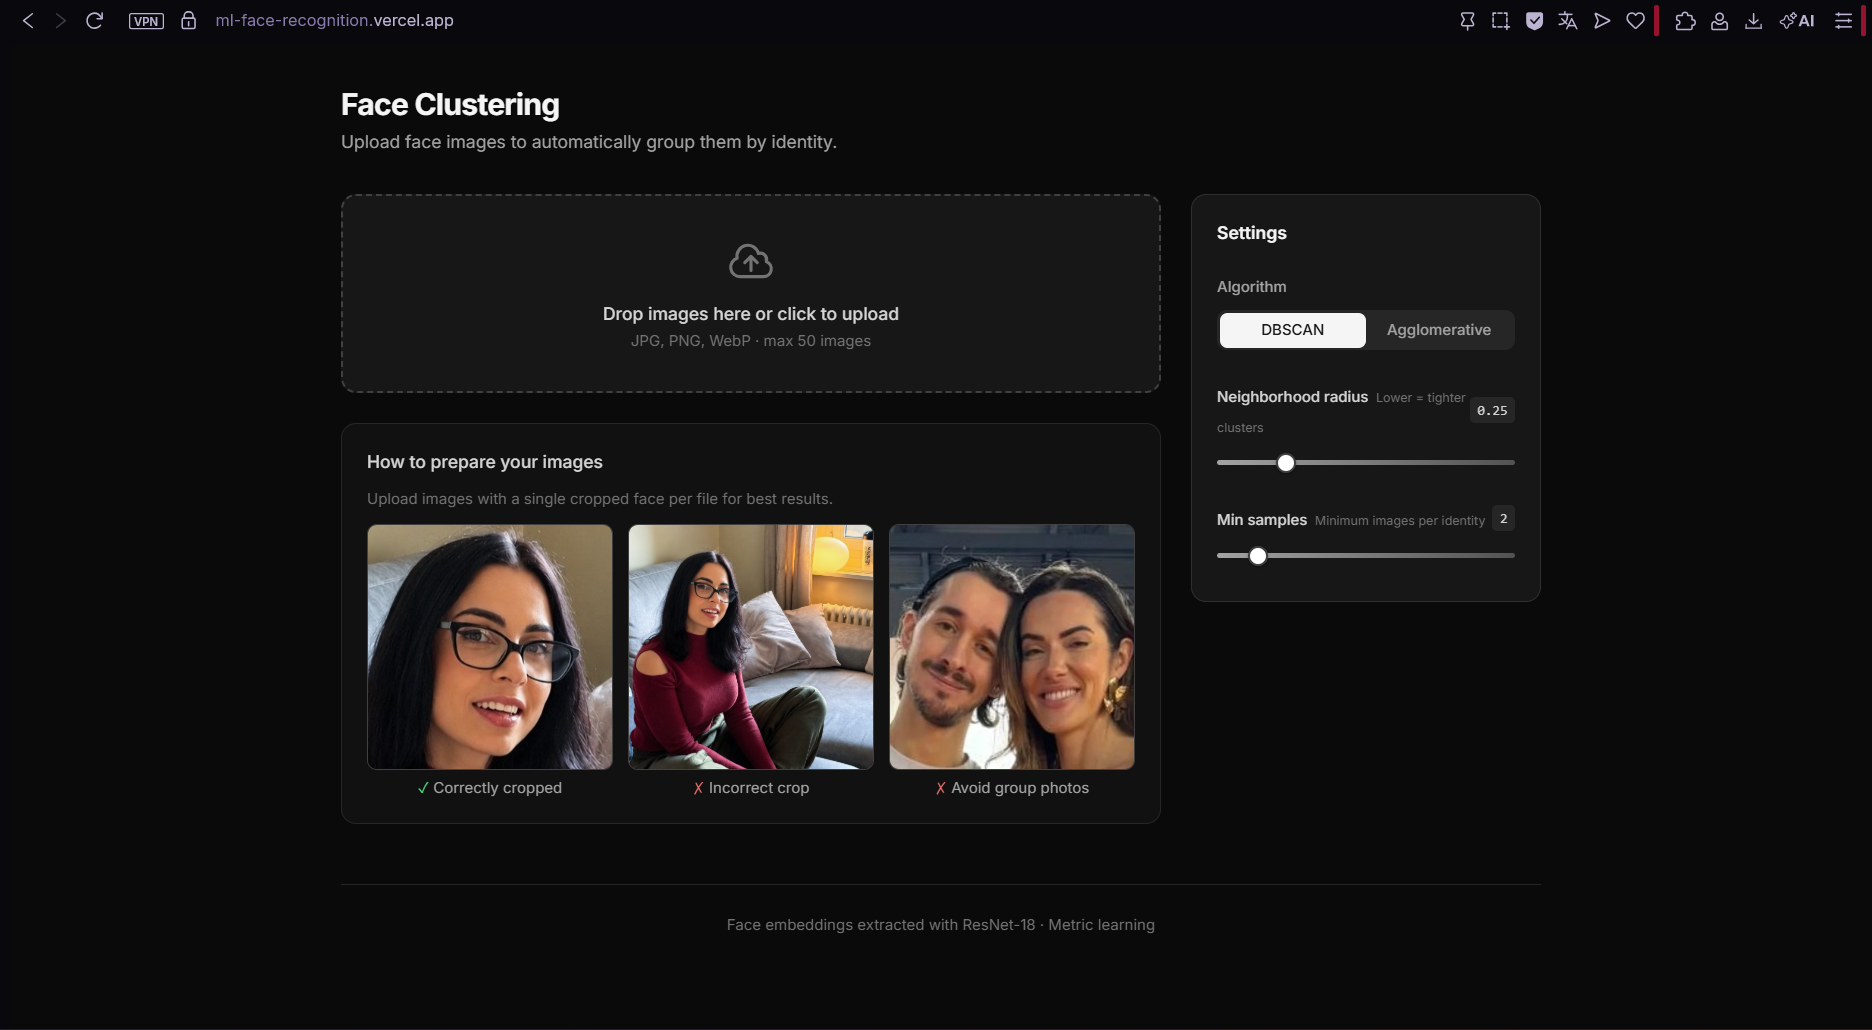
\includegraphics[width=0.85\linewidth, height=4.5cm, keepaspectratio]{website.png}\\[0.8em]
\href{https://clusteringdemo.vercel.app}{\color{colAccent}\textbf{\large clusteringdemo.vercel.app}}
\end{frame}

\end{document}
